\documentclass[a4paper,12pt]{llncs}
\usepackage[top=75pt, bottom=75pt, left=85pt, right=85pt]{geometry}

\usepackage{amssymb}
\setcounter{tocdepth}{3}
\usepackage{graphicx}
\usepackage{soul,color}
\usepackage{url}
\usepackage{algorithm}
%\usepackage{enumitem}
\newcommand{\keywords}[1]{\par\addvspace\baselineskip
\noindent\keywordname\enspace\ignorespaces#1}
\newcommand{\ie}{i.e.} 
\newcommand{\eg}{e.g.} 
\newcommand{\et}{et al. }

\begin{document}
\title{Weekly Report -- 50}
\author{Xiufeng Liu}
\institute{University of Waterloo, CA\\
\email{xiufeng.liu@uwaterloo.ca}
}
\maketitle


\section{This Week}
At the beginning of this week, I first investigated the SciDB on how it can fit our benchmark requirements. I designed a three-dimensional data model for ESSEX power dataset,  import the data set, and learn how to do the basic data analysis in SciDB. In the later of this week, I focus on the study of the use of KDB+, a column-oriented in-memory database.

\section{Next Week}
Learn the q programming language, and try to write the program for the  analysis data model.

\section{SciDB}
\subsection{Introduction}
\label{sec:scidb}
SciDB is an open source science-oriented DBMS that provides massively scalable complex data analysis. It supports versioning, provenance, parallel computation on shared-nothing cluster, user-defined functions (UDFs) and uncertainty queries. 

{\bf Data model:} Unlike conventional relational databases, SciDB uses an array data model that provides compact data storage and high performance on ordered data, such as temporal data, spatial data, and matrix-based data for linear algebra operations \cite{scidb}.  An array has a name and the schema that describes the structure of the array. The schema contains the information of array attributes and dimensions. The combination of dimensions form the cells each of which contains the values of one or multiple attributes, or even another array. A dimension consists of a list of indexed values, and the number of index values in a dimension is referred as the size of the dimension. Therefore, the attribute values (in cells) can be quickly located by the dimensions. The format of dimension declaration is \emph{[name\_of\_dimension=start\_index:end\_index, chuck\_size, chuck\_overlap]}. Figure~\ref{fig:essexdatamodel} shows the script of creating an array for storing ESSEX data, and the visualized data model.  This data model has three dimensions \texttt{timestamp, household,} and \texttt{temperature}, and one attribute, \ie, \texttt{reading}. SciDB also supports ragged dimensions, \eg, in a 2D array, the number of columns for the rows are not all equal. 

\begin{figure}[htp]
\begin{minipage}{0.5\textwidth}
{\scriptsize
\begin{verbatim}
CREATE ARRAY essex<reading:double> [
       time=0:*,100,0,
       household=0:*,100,0,                       
       temperature=0:*,200,0
]
\end{verbatim}
}
\end{minipage}
\begin{minipage}{0.5\textwidth}
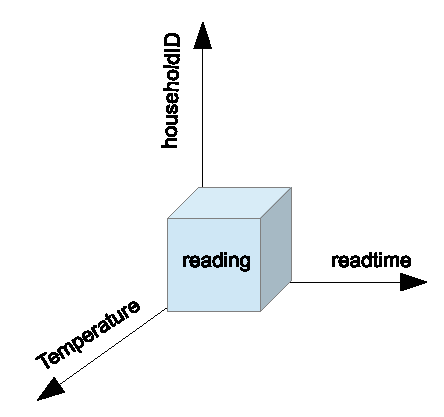
\includegraphics[width=0.5\textwidth]{images/scidbdatamodel}
\end{minipage}
\caption{Data model for storing ESSEX data}
\label{fig:essexdatamodel}
\end{figure}


 

{\bf Languages and UDFs:}
SciDB supports two types of languages: Array Query Language (AQL) and Array Functional Language (AFL). AQL is declarative SQL-like language extended to work with array data, while AFL is a functional language for the internal implementation of operators. The two languages can be switched freely in the SciDB client, \texttt{iquery}. SciDB currently provides a number of array-specific  operators, including \texttt{Aggregate, Apply, Filter, Join, Regrid, Subsample}, and the operations for linear algebraic and matrix including clustering, coverariance, linear and logistic regression. Users can also define their own Postgres-style functions (UDFs) to enhance an array. For example, UDFs (for  scaling, transformation, translation, etc) can be defined to the dimensions of an array to form a new coordinate system. 

{\bf Distributed computing:} SciDB is built on the concept of shared-nothing architecture deployed up to thousands of nodes. It employs {\em master-slaves} architecture (see Figure~\ref{fig:scidbcluster}), which the supervisor (master node) is responsible for dispatching queries and coordinating the execution among the slave nodes, and each of the slave nodes processes the data on its local storage. SciDB uses PostgreSQL to store the data catalogue. Figure~\ref{fig:scidbcluster}  shows a schematic view of a cluster with five SciDB instances \cite{scidbuserguide}. The SciDB client interacts with the coordinate instance, and the coordinate communicate with the other four slave instances to distribute data and computational load \cite{brown2010}. 

\begin{figure}[htp]
\centering
\includegraphics[width=250 px]{images/scidbcluster}
\caption{SciDB architecture on a cluster}
\label{fig:scidbcluster}
\vspace{-10pt}
\end{figure}





\subsection{Overview of Benchmark Study}
Figure~\ref{fig:scidbbenchmarksystem} illustrates the overview of benchmark study as well as the data flow from through the system components. The data sets include the ESSEX power data provided by Waterloo utility company, and the weather data of Waterloo region. The original data sets are imported into MySQL database, and pre-processed by co-relating the meter readings and the temperature when the meter was read. The pre-processed data containing the meter readings, timestamps, meter ID (or household ID), and temperatures, are exported to a comma-separated-values text files (CSV). This CSV file is then processed to SciDB dense load format (DLF) by the tool, \texttt{csv2scidb}, shipped with SciDB.  This load format is used when the attributes of every cell in the array have values, and no cell is allowed to be empty (but the attribute values in a cell can be null).  Our aim is to load the data into the multidimensional array in the SciDB (see the data model in Figure~\ref{fig:essexdatamodel}), however, the tool \texttt{csv2scidb}  only supports generating one-dimensional load format. Therefore, we first create a temporary on-dimensional array in the SciDB,  load the generated DLF file into this temporary array, and finally use the function \texttt{redimension\_store} to transform from one-dimension to multi-dimension array.  Since our data is stored in the three-dimension data model, which is sparse \eg, the data on the temperature dimension is not continuous. This process greatly simplifies the loading, although SciDB supports the sparse load format (SLF), which users can explicitly specify the coordinate of the cell of the data to be loaded into. When the data has been loaded, we can   aggregate the data from different dimensions. The analysis results are saved in the SciDB, then exported to visualize in the analysis visualization tools, such as Matlab and R. Currently, SciDB R package \cite{scidbr} is available for using R directly to analysis the data from SciDB.  The data transferring  between SciDB and R is over HTTP. 

\begin{figure}[htp]
\centering
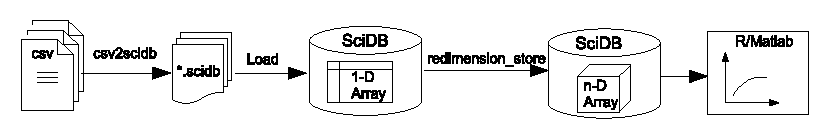
\includegraphics[width=370 px]{images/scidbbenchmarksystem}
\caption{System architecture of the benchmark study using SciDB}
\label{fig:scidbbenchmarksystem}
\vspace{-10pt}
\end{figure}



\subsection{Analytics Schema}
Figure~\ref{fig:essexdatamodel} has shown our analytics schema, an array with one attribute \texttt{reading}, and three dimensions, \texttt{time, household} and \texttt{temperature}. According to the SciDB user guide \cite{scidbuserguide}, when each chunk is roughly 10 to 20 MB of data, queries can have an optimal performance. Therefore, considering the array on \texttt{temperature} dimension is sparse, we set its chunk size to 200 while the other two dimension as 100. There is no overlap between chunks, which the values is set to 0. 

\section{KDB+}
kdb+ is the single-platform, high-volume, and high-performance database which supports billions of real-time records analysis \cite{kdb}. kdb+ has an enterprise 64-bit version, and an 32-bit trial version. However,  a full-64bit version can be made available for academic users. Kdb+ is an in-memory column-oriented database based on the concept of ordered lists, which makes it extremely fast to do data analytics. Kdb+ is able to capturing, managing, and analyzing billions of real-time ticks,  and kdb+tick processes millions of records per second. It is now widely used by the companies in financial services industry, including Goldman Sachs, Morgan Stanley, Deutsche Bank, etc. \cite{kdbusers}, to capture real-time ticks and do analysis.

Unlike conventional row-based DBMS, kdb+ is column-oriented database which data is stored in vectors of ordered lists, instead of the set as in RDBMS. Therefore, multiple identical values can co-exists in a list. Since kdb+ is an in-memory database, it requires a lot of RAM if keeps all the column data of a massive table  in memory. Therefore,  a big table can be splayed (partitioned), and only the necessary column data is read and kept in memory. This minimizes the memory foot print and improves the performance greatly during data analysis. If the size of one-column data still cannot fit into memory, the data can be further partitioned horizontally, for example horizontally partition based on the date of time series data. The data file for each partition is stored under a separate folder in file system.

Q language servers as the query language for kdb+, which was developed by Arthur Whitney.  Q is a interpreted vector based dynamically typed language  built for speed and expressiveness. Since q is interpreted, users can enter commands straight into the console, do not have to wait for compilation, and the results can be returned instantaneously. Since the tables in kdb+ are columns of vectors, q language can be used as easily on table data as it was on lists. The backbone of the q language is  atoms, lists, dictionaries and tables. 

 
\medskip
\begin{thebibliography}{1}

\bibitem{ibmbenchmark}
Ten Million Meters Scalable to One Hundred Million Meters for Five Billion Daily Meter Readings. Sept. 2011.

\bibitem{yang}
J.~Yang, Y.~Zhai, D.~Xu, et al. ``SMO Algorithm applied in
time series model building and forecast". In {\em Proc. of ICMLC}, 2007:2395-2400, 2012.

\bibitem{brown2010}
P.~G.~Brown.  ``Overview of SciDB: Large Scale Array Storage, Processing and Analysis". In Proc. of SIGMOD, pp. 963--968, 2010.

\bibitem{scidbuserguide}
SciDB User's Guide. \url{http://scidb.org/HTMLmanual/13.3/scidb_ug/index.html}

\bibitem{scidb}
SciDB \url{http://www.scidb.org/} as of 2013-12-07.

\bibitem{scidbr}
SciDBR. \url{https://github.com/Paradigm4/SciDBR} as of 2013-12-07.

\bibitem{kdb}
KDB+.  \url{www.kx.com} as of 2013-12-07.

\bibitem{kdbusers}
KDB+ Customers. \url{http://kx.com/end-user-customers.php}
\end{thebibliography}



\end{document}
